\documentclass[aspectratio=169]{beamer}
\usepackage[utf8]{inputenc}
\usepackage{lmodern}
\usepackage{tikz}
\usepackage{hyperref}
\definecolor{pbprimary}{HTML}{F4A261}
\definecolor{pbsecondary}{HTML}{FFE8B6}
\setbeamercolor{palette primary}{bg=pbprimary, fg=white}
\setbeamercolor{frametitle}{fg=pbprimary}
\setbeamercolor{title}{fg=pbprimary}
\setbeamercolor{block title}{bg=pbprimary, fg=white}
\setbeamercolor{block body}{bg=pbsecondary, fg=black}
\setbeamercolor{alertblock title}{bg=pbprimary, fg=white}
\setbeamercolor{alertblock body}{bg=pbsecondary!80, fg=black}
\setbeamertemplate{navigation symbols}{}
\setbeamertemplate{itemize item}{\color{pbprimary}\Large$\blacktriangleright$}
\title{Tasks \& Technology Build A House}
\subtitle{Student Guide Deck}
\author{Pine Brook IGNITE}
\date{Spring 2026}
\begin{document}
\begin{frame}[plain]
\begin{center}
{\usebeamerfont{title}\color{pbprimary}\Huge Tasks \& Technology Build A House\par}
\vspace{0.3cm}
{\Large Today we will learn, build, test, and show our thinking.\par}
\vspace{0.35cm}
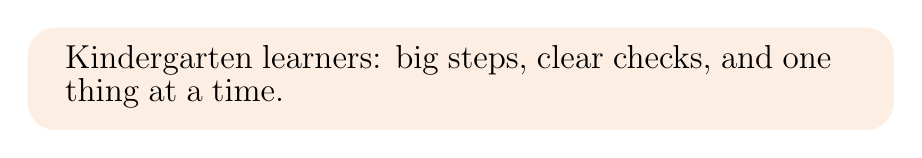
\begin{tikzpicture}
\fill[pbprimary!18, rounded corners=10pt] (0,0) rectangle (11,1.3);
\node[anchor=west, text width=10.2cm] at (0.35,0.68) {\large Kindergarten learners: big steps, clear checks, and one thing at a time.};
\end{tikzpicture}
\end{center}
\end{frame}
\begin{frame}{Todays Goal}
\begin{itemize}
\item I can tell you what the word technology means
\item I can tell you what the word task means
\item I can give an example of a task that is completed with and without computing technology (K-1.IC.1)
\end{itemize}
\begin{block}{Remember}
We do not have to be perfect right away. We take one step, then the next step, then we check.
\end{block}
\end{frame}
\begin{frame}{What You Need}
\begin{itemize}
\item Your class materials
\item The digital tool or build materials for today
\item A partner voice and your thinking
\end{itemize}
\begin{block}{Partner Norms}
Look. Listen. Try. Talk. Help without taking over.
\end{block}
\end{frame}
\begin{frame}{Step 1}
\begin{block}{Look at the challenge and name the goal.}
Look at the challenge and name the goal.
\end{block}
\begin{itemize}
\item Point to the part that tells you what success means.
\item Make the challenge criteria visible from the first slide through cleanup.
\end{itemize}
\centering\large\color{pbprimary} Pause. Check. Then move on.
\end{frame}
\begin{frame}{Step 2}
\begin{block}{Build, test, and notice what happens.}
Build, test, and notice what happens.
\end{block}
\begin{itemize}
\item Change one thing at a time so your next move is clear.
\item Break the design process into plan, build, test, and improve rather than one big make.
\end{itemize}
\centering\large\color{pbprimary} Pause. Check. Then move on.
\end{frame}
\begin{frame}{Step 3}
\begin{block}{Improve your design and explain your thinking.}
Improve your design and explain your thinking.
\end{block}
\begin{itemize}
\item Tell what worked, what did not yet work, and what you tried next.
\item Use teacher talk that celebrates revision so early failure feels normal.
\end{itemize}
\centering\large\color{pbprimary} Pause. Check. Then move on.
\end{frame}
\begin{frame}{If You Get Stuck}
\begin{enumerate}
\item Read the directions on your screen or slide one more time.
\item Check the example, the checklist, or your partner role.
\item Try one small change before asking for a full rescue.
\item Students may rush into building before naming the target or the constraint.
\end{enumerate}
\begin{alertblock}{Help Routine}
Stop. Breathe. Point to where you are stuck. Ask a specific question.
\end{alertblock}
\end{frame}
\begin{frame}{Show Your Learning}
\begin{itemize}
\item I stayed with the steps and used the help routine when I needed it.
\item I made, coded, explained, or revised something that matches the lesson goal.
\item I can point to one choice, fix, or idea I learned today.
\end{itemize}
\begin{block}{Before You Leave}
Save it, share it, explain it, or demonstrate it.
\end{block}
\end{frame}
\begin{frame}{Teacher Voiceover Cues}
\footnotesize
\begin{itemize}
\item Today we are working on tasks \& technology build a house. Watch first, then try it with me.
\item If you feel stuck, stop at the checkpoint slide and use the help routine before you panic.
\item Show what you learned by saving, sharing, explaining, or demonstrating one clear success move.
\end{itemize}
\color{gray}This slide can be removed before student use if you only want the visual deck.
\end{frame}
\end{document}
